\anexo{Pantallas y wireframes de Allocia}\label{annex:wireframes}

Este anexo completa la Subsección~\ref{sec:pantallas} con las pantallas del cliente web que no aparecen en el cuerpo del Proyecto y con los wireframes de alta fidelidad del diseño original, en formato móvil, elaborados con Stitch (Google). Las capturas provienen de una cuenta de prueba con ocho posiciones, con el correo difuminado donde aparece: acceso y registro (Figura~\ref{fig:anx-acceso}), el cliente web en el navegador de un teléfono (Figura~\ref{fig:anx-web-movil}), política de privacidad y cuenta con exportación y baja (Figura~\ref{fig:anx-privacidad}), desglose y detalle por activo (Figura~\ref{fig:anx-desglose}), alertas e informe (Figura~\ref{fig:anx-alertas}) y ajustes (Figura~\ref{fig:anx-ajustes}). En la Figura~\ref{fig:anx-acceso}, las tarjetas de la ilustración lateral son de demostración.

\section*{Pantallas del cliente web}
\begin{figure}[ht]
	\centering
	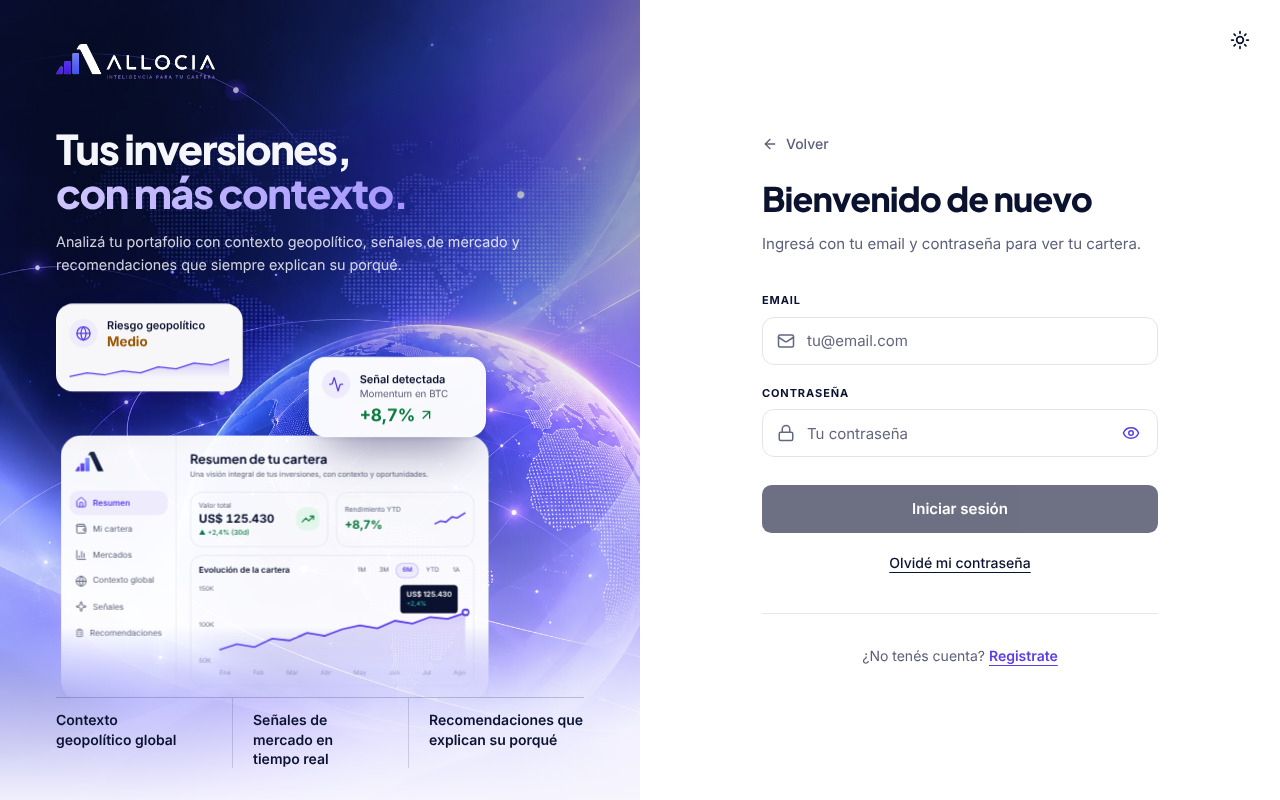
\includegraphics[width=0.485\textwidth]{figures/pantallas/web/a-02-login.png}\hfill
	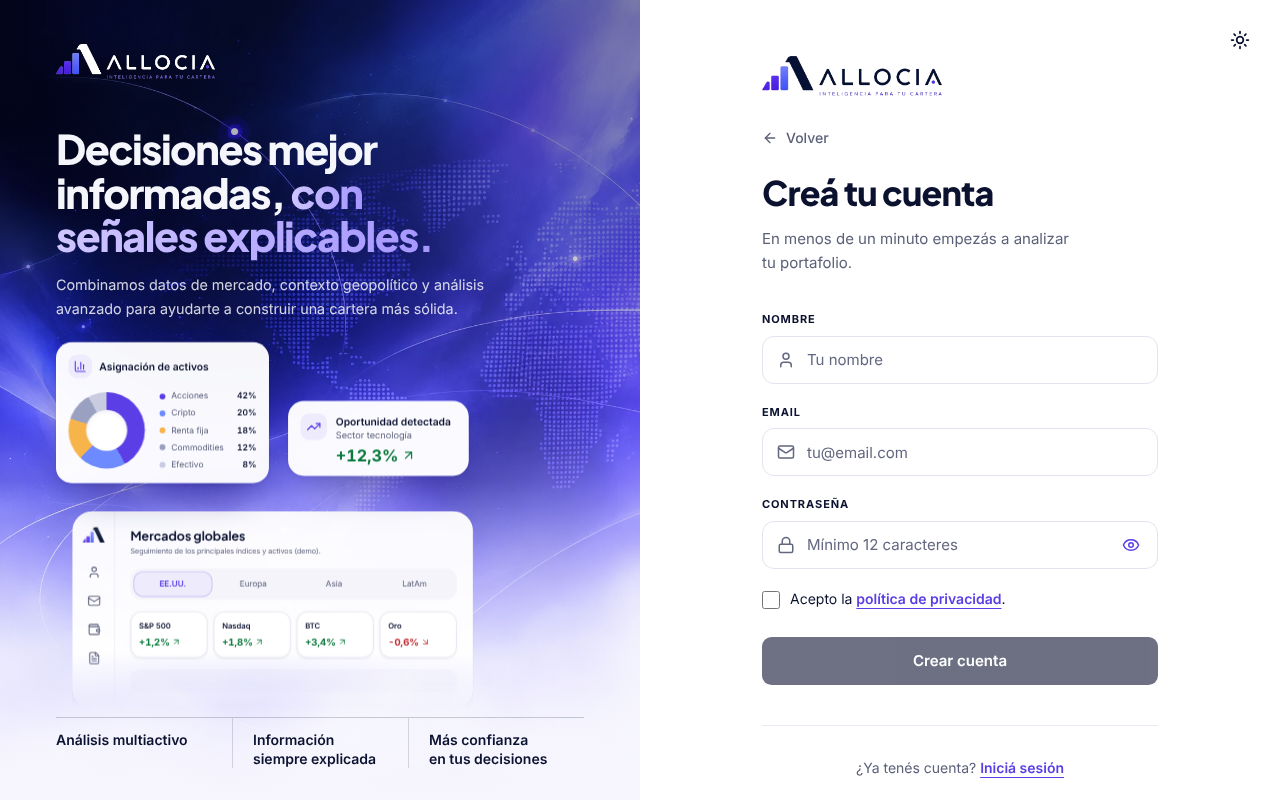
\includegraphics[width=0.485\textwidth]{figures/pantallas/web/a-03-registro.png}
	\caption{Capturas del inicio de sesión y del registro. Fuente: elaboración propia.}\label{fig:anx-acceso}
\end{figure}

\section*{Cliente web en el teléfono}
El cliente web adapta su diseño a la pantalla de un teléfono: el menú lateral se reemplaza por una barra de pestañas inferior y las tarjetas se apilan en una sola columna. La Figura~\ref{fig:anx-web-movil} muestra Resumen, Riesgo y Señales en el navegador de un teléfono, sin la aplicación instalada.
\begin{figure}[ht]
	\centering
	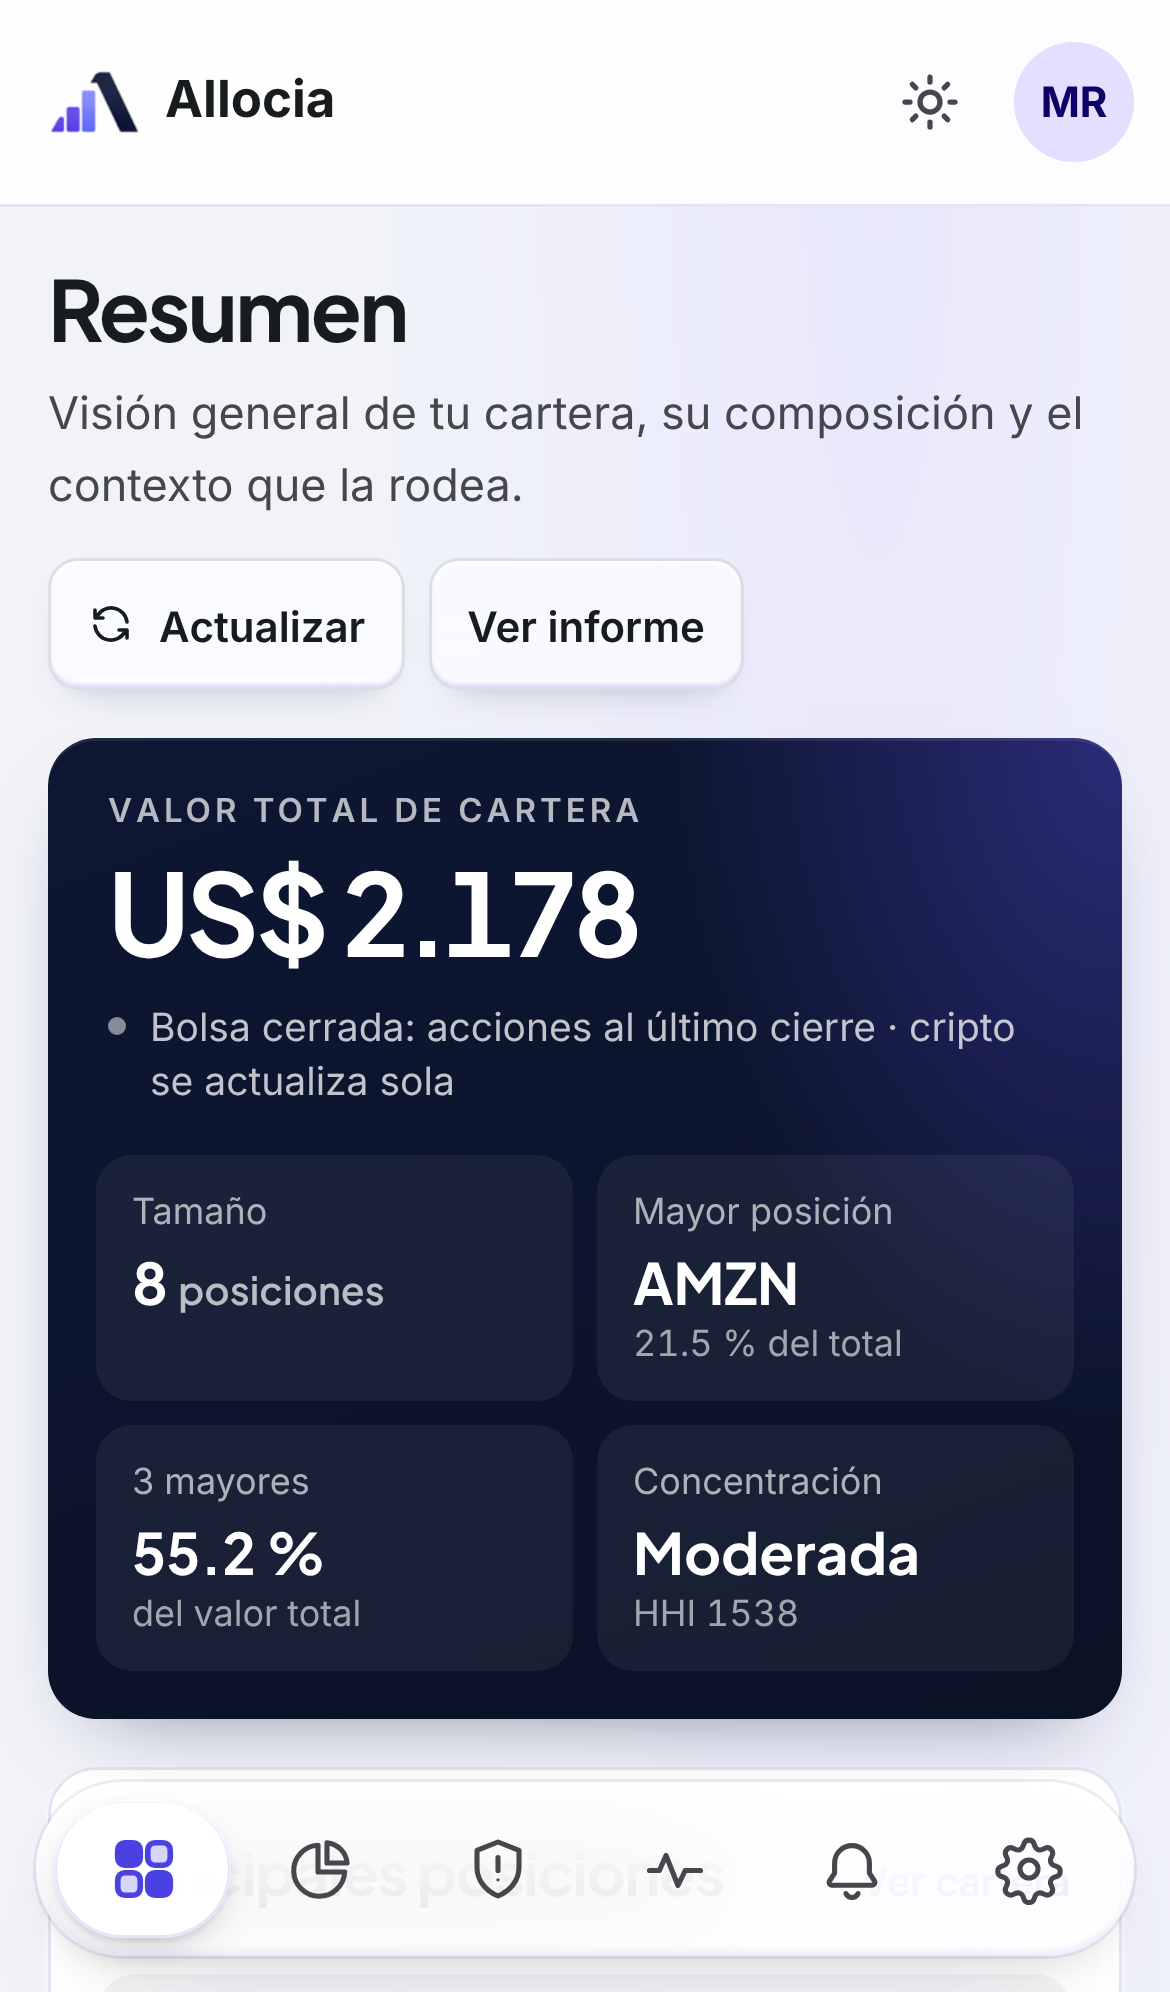
\includegraphics[height=7.4cm]{figures/pantallas/web/m-01-resumen.png}\hspace{4pt}
	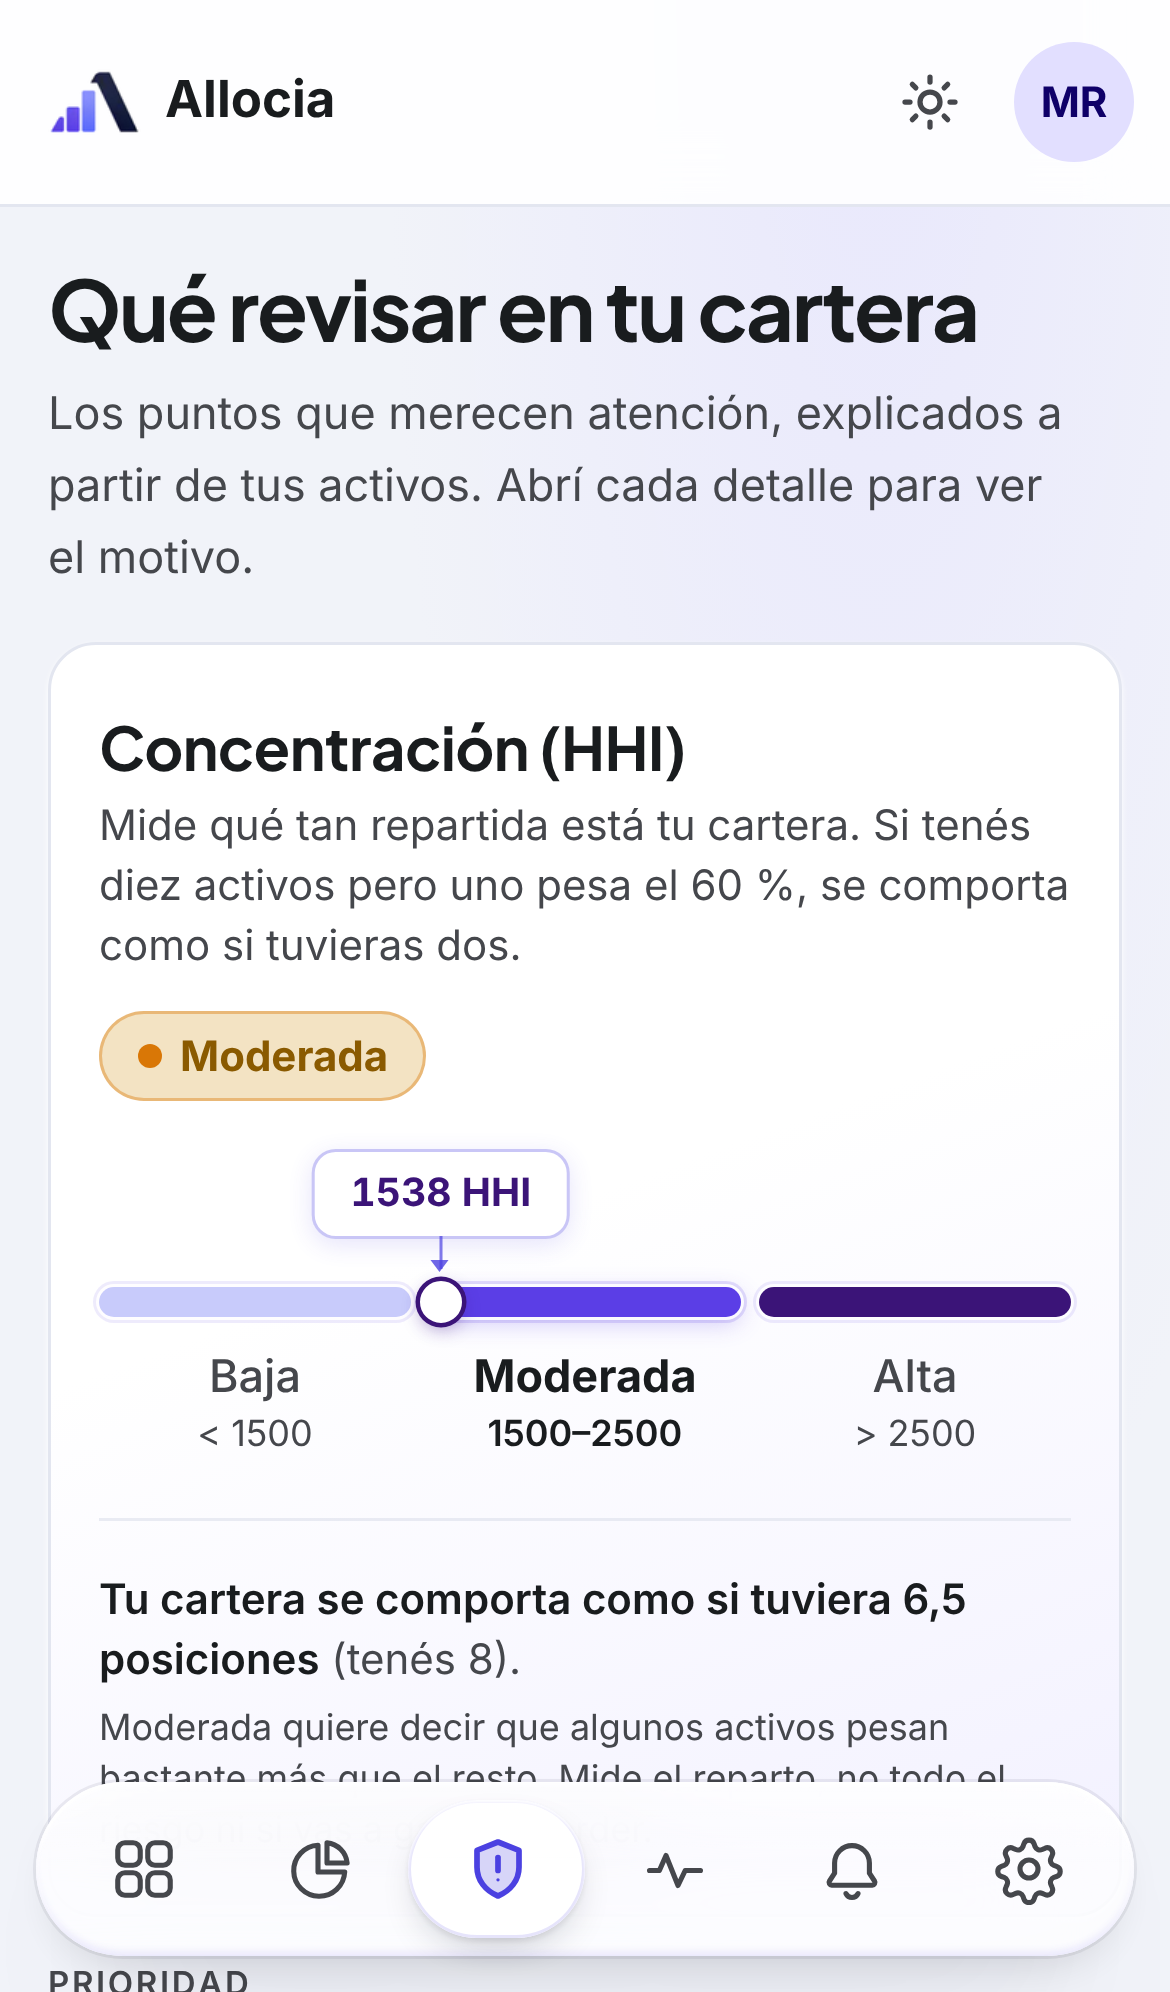
\includegraphics[height=7.4cm]{figures/pantallas/web/m-02-riesgo.png}\hspace{4pt}
	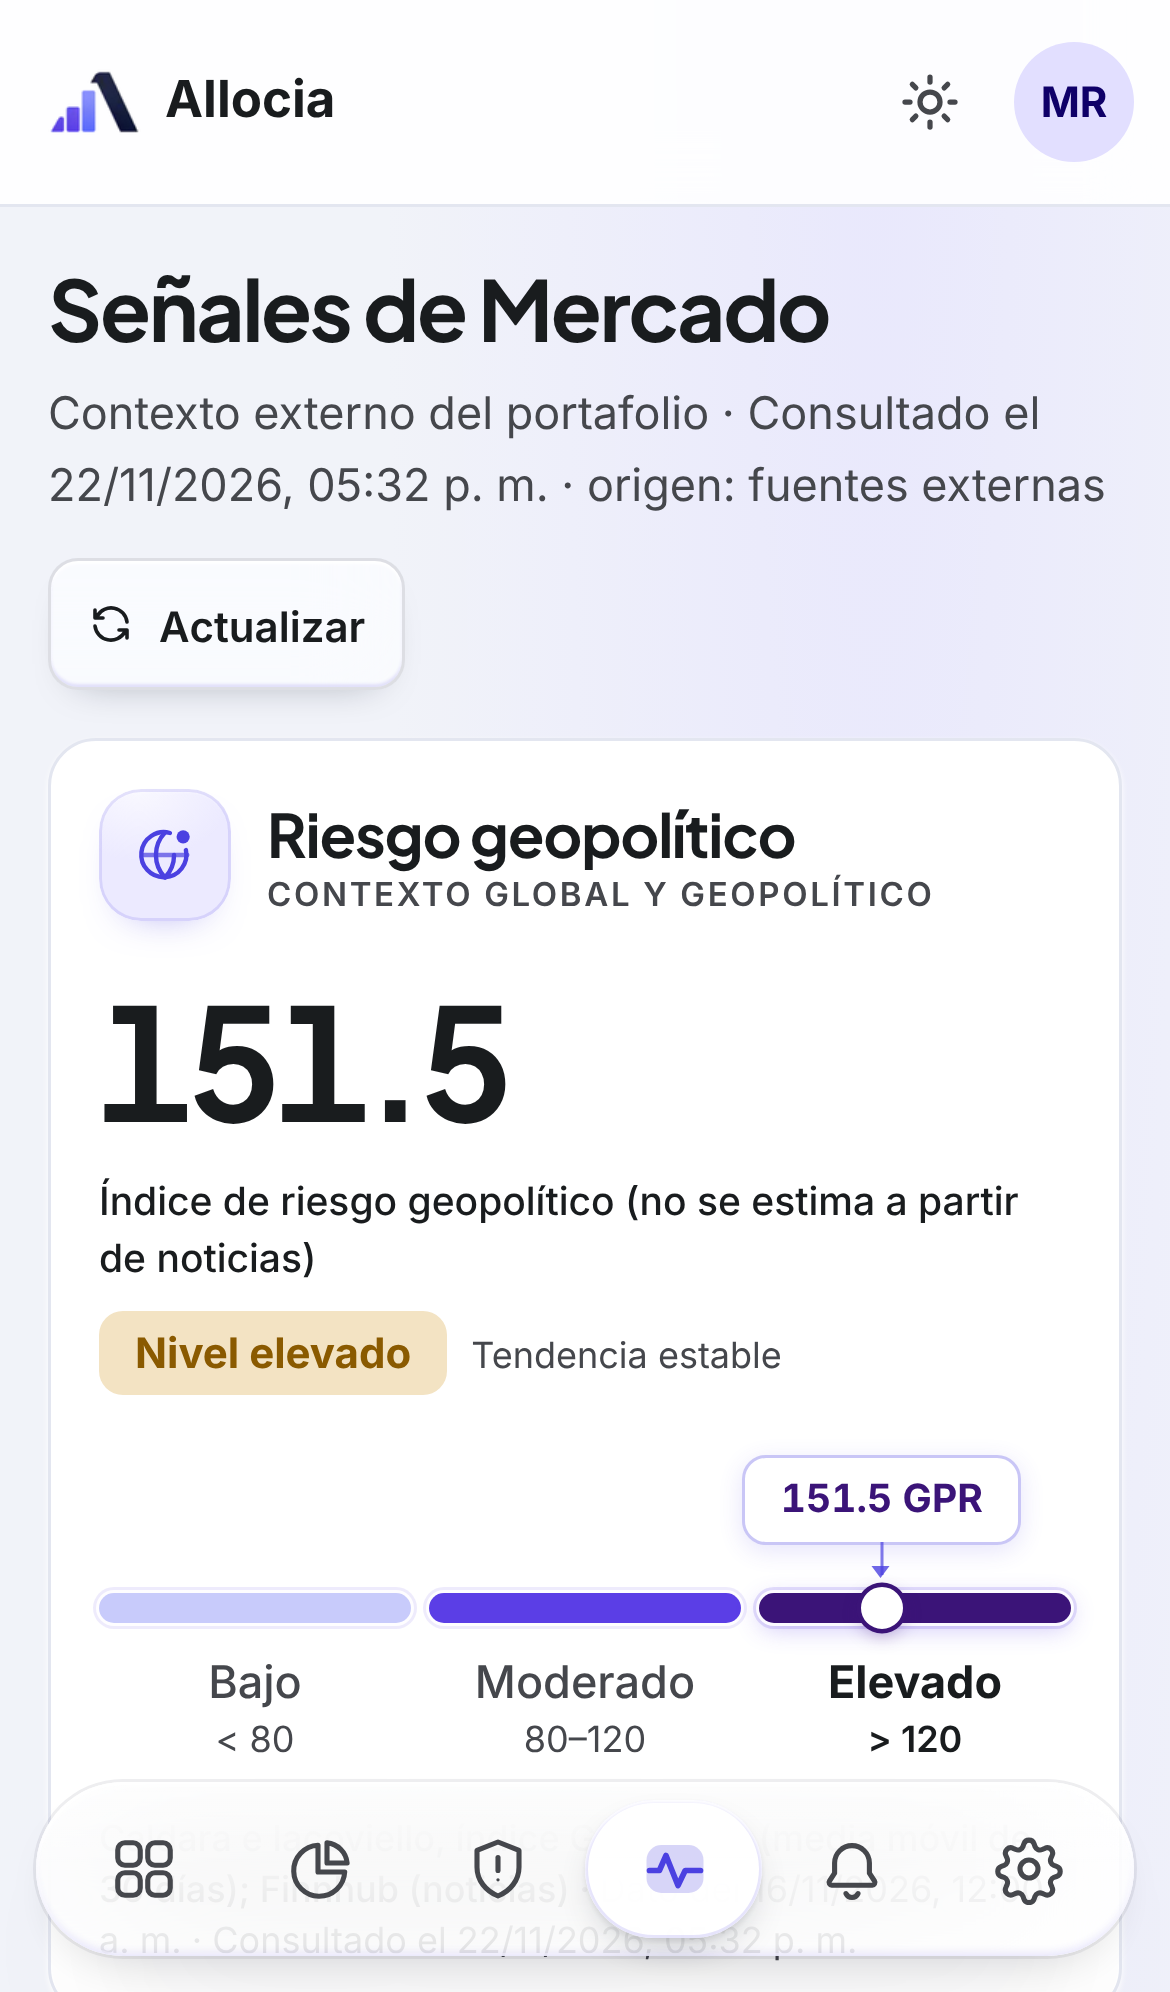
\includegraphics[height=7.4cm]{figures/pantallas/web/m-03-senales.png}
	\caption{Capturas del cliente web en el navegador de un teléfono: Resumen, Riesgo y Señales. Fuente: elaboración propia.}\label{fig:anx-web-movil}
\end{figure}

\section*{Privacidad y baja de cuenta}
La política de privacidad indica quiénes son los responsables, con qué finalidad se tratan los datos, cuáles se tratan, cuánto tiempo se guardan y qué derechos tiene la persona. La pantalla de cuenta permite exportar los datos y pedir la baja confirmando la contraseña (RF9 y RF10). La propia política aclara que un responsable legal debe revisarla antes de publicar el servicio.
\begin{figure}[ht]
	\centering
	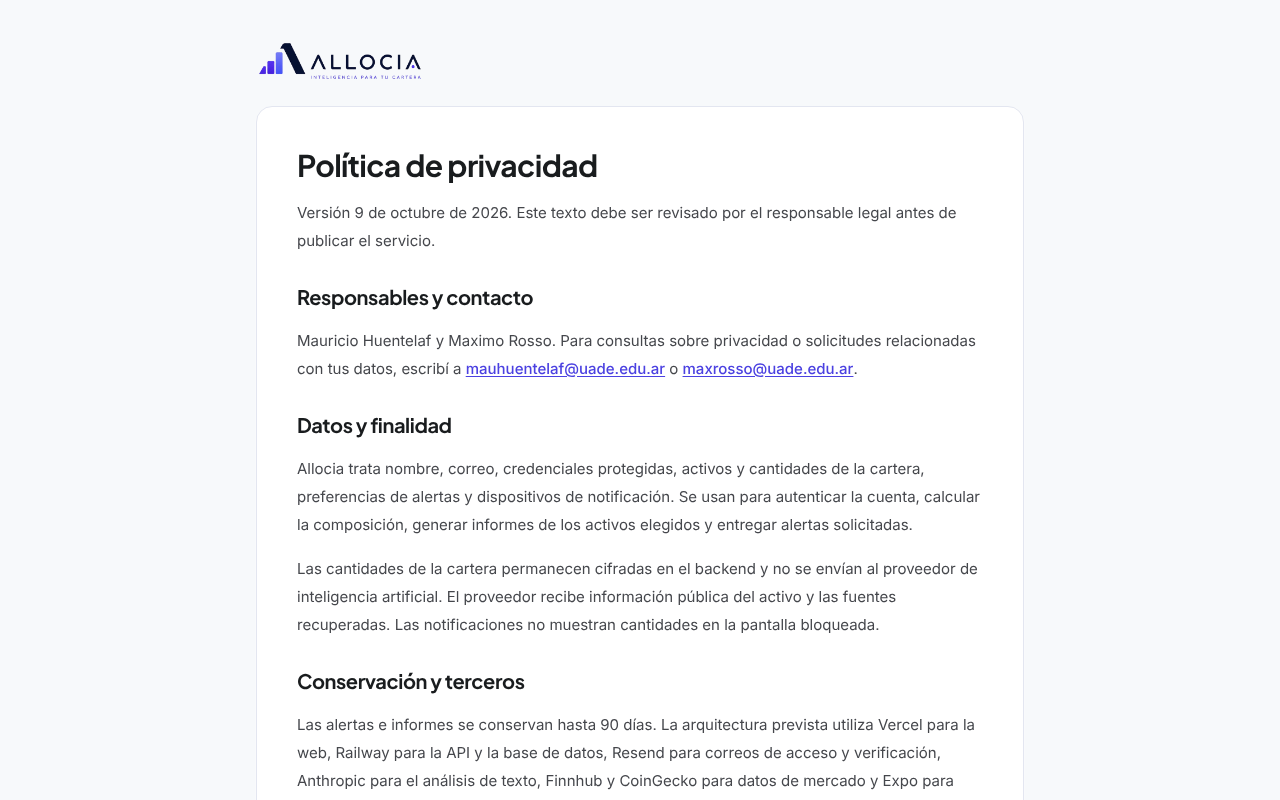
\includegraphics[width=0.82\textwidth]{figures/pantallas/web/a-04-privacidad.png}\\[6pt]
	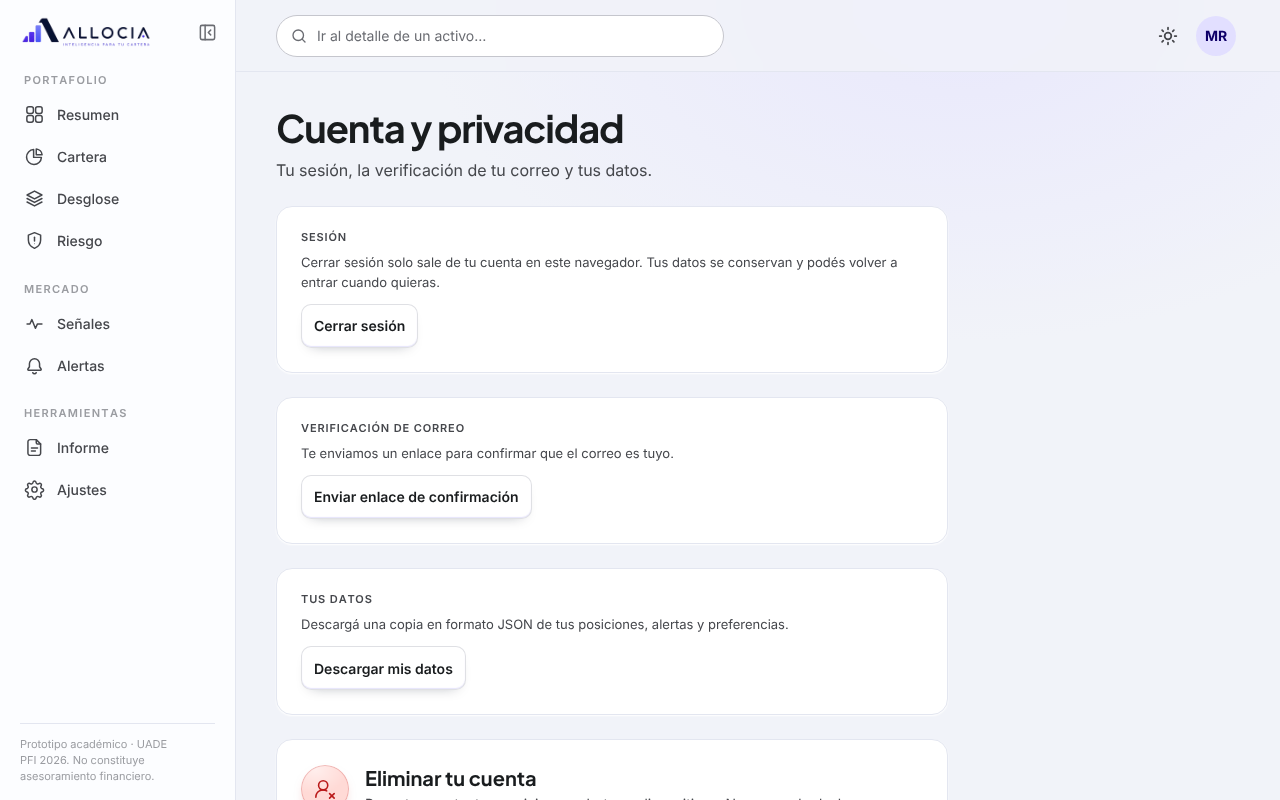
\includegraphics[width=0.82\textwidth]{figures/pantallas/web/a-10-cuenta.png}
	\caption{Capturas de la política de privacidad y de la pantalla de cuenta, con exportación y baja. Fuente: elaboración propia.}\label{fig:anx-privacidad}
\end{figure}

\begin{figure}[ht]
	\centering
	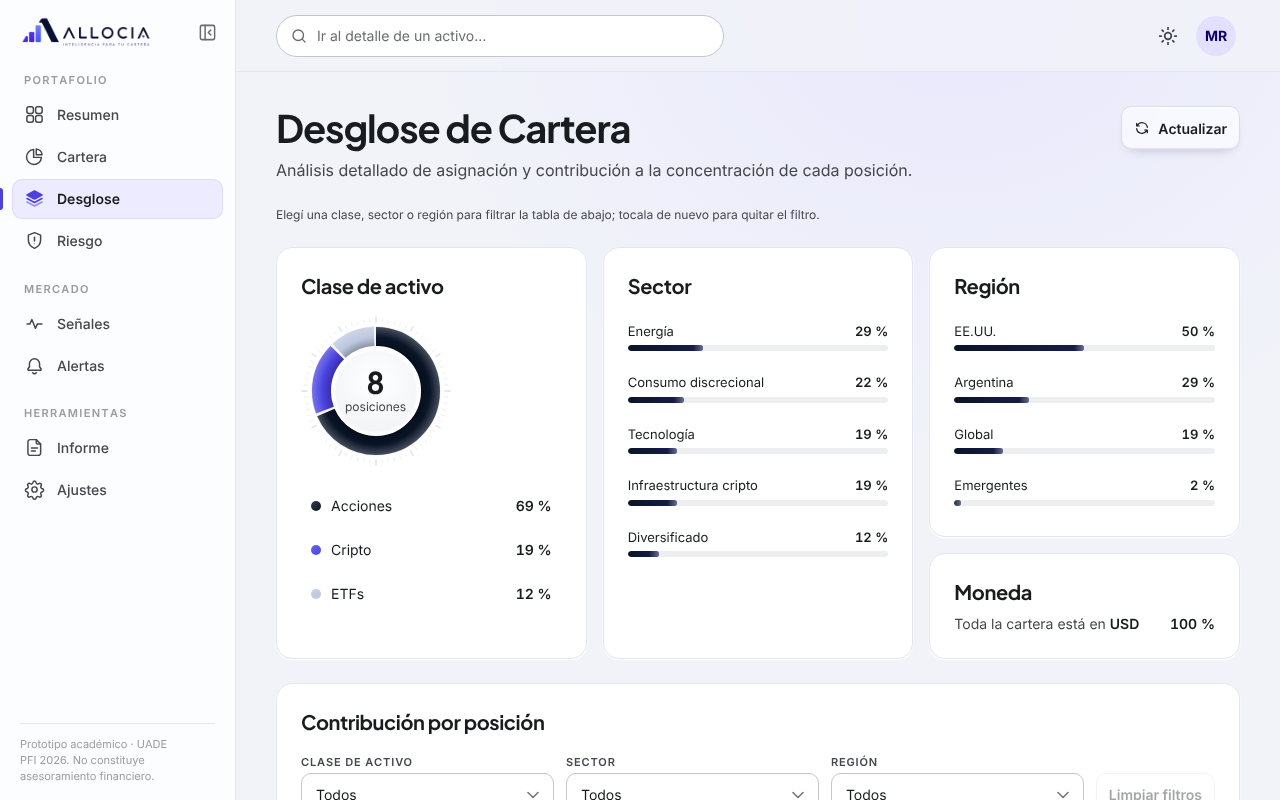
\includegraphics[width=0.82\textwidth]{figures/pantallas/web/a-05-desglose.png}\\[6pt]
	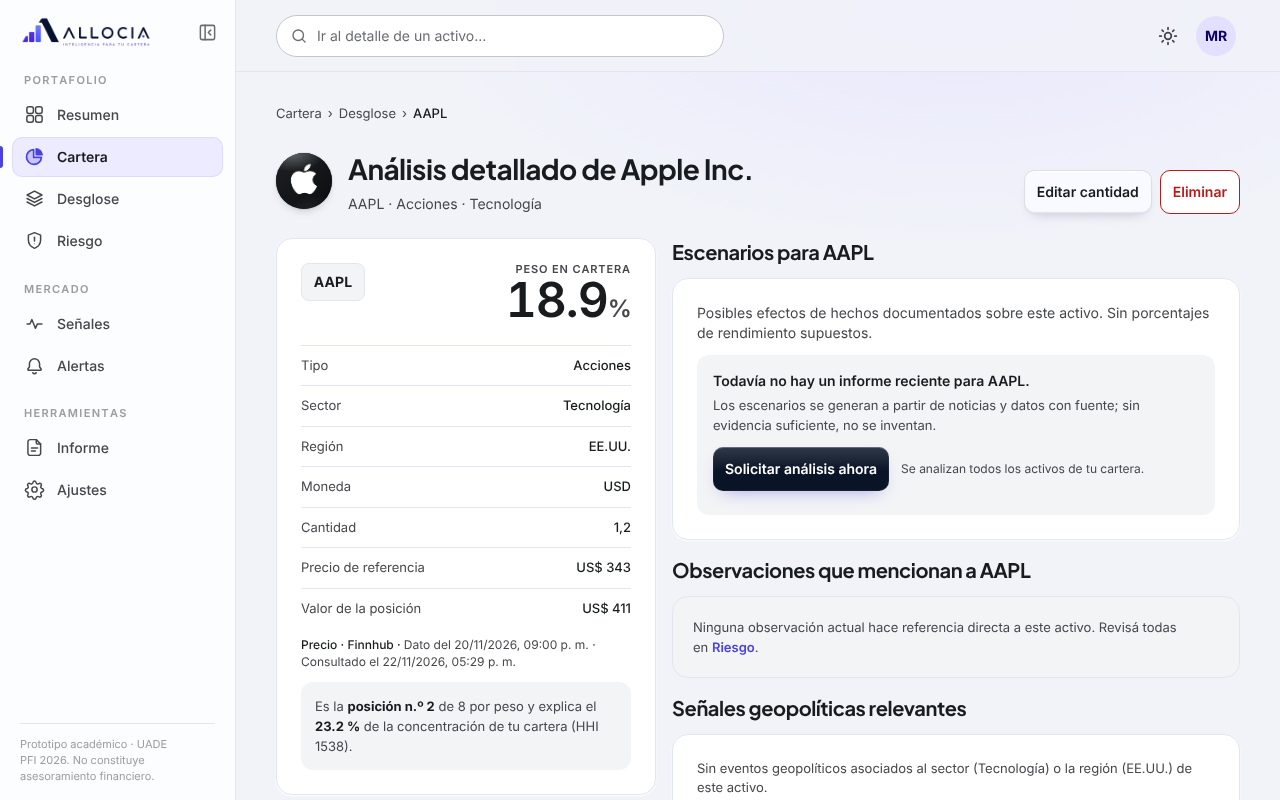
\includegraphics[width=0.82\textwidth]{figures/pantallas/web/a-06-detalle.png}
	\caption{Capturas del desglose de la cartera y del detalle de un activo. Fuente: elaboración propia.}\label{fig:anx-desglose}
\end{figure}

\begin{figure}[ht]
	\centering
	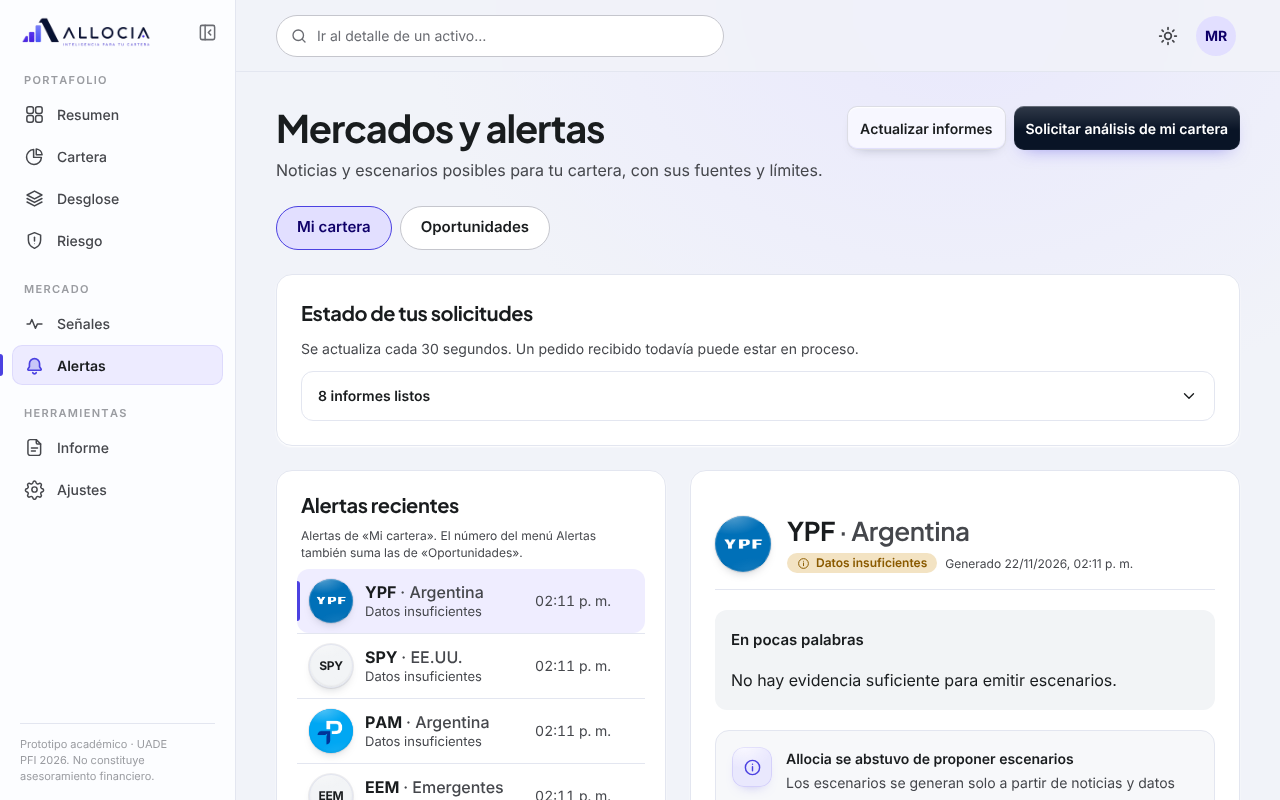
\includegraphics[width=0.82\textwidth]{figures/pantallas/web/a-07-alertas.png}\\[6pt]
	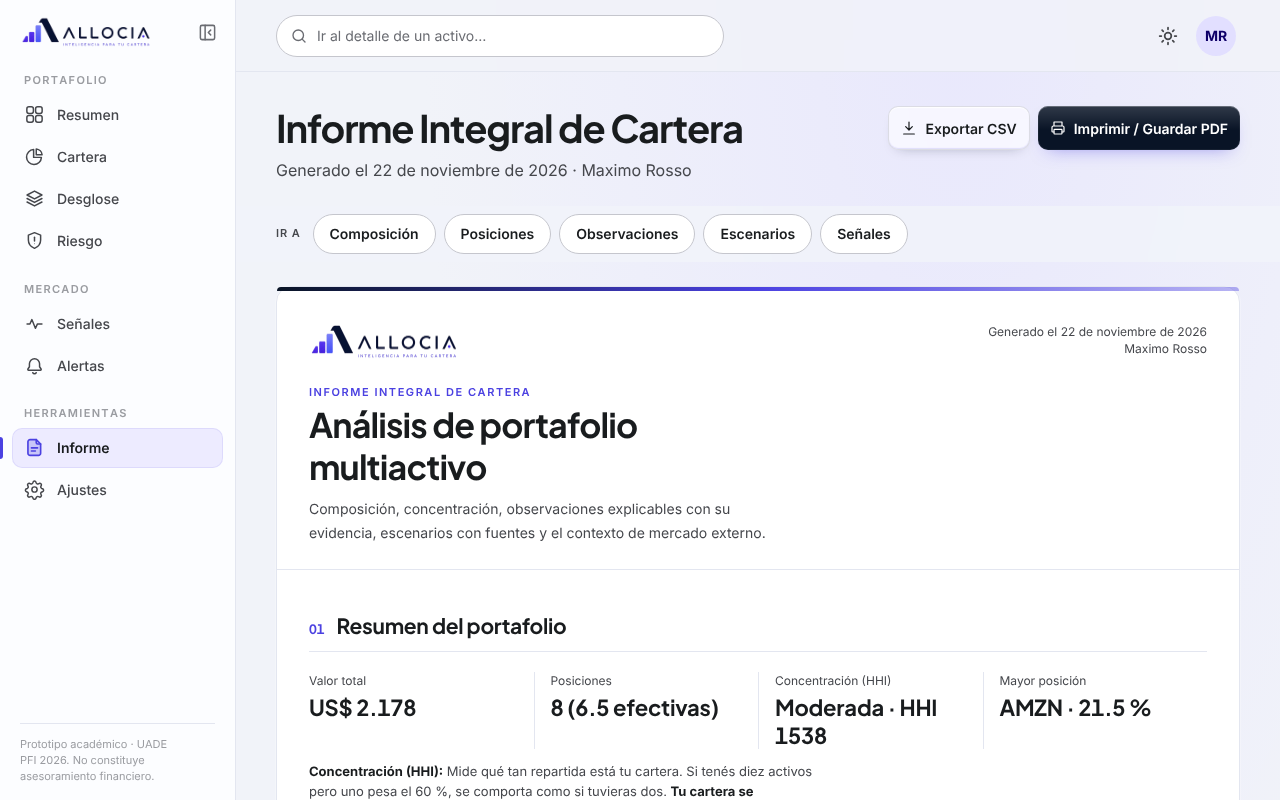
\includegraphics[width=0.82\textwidth]{figures/pantallas/web/a-08-informe.png}
	\caption{Capturas de mercados y alertas, y del informe de la cartera. Fuente: elaboración propia.}\label{fig:anx-alertas}
\end{figure}
\begin{figure}[ht]
	\centering
	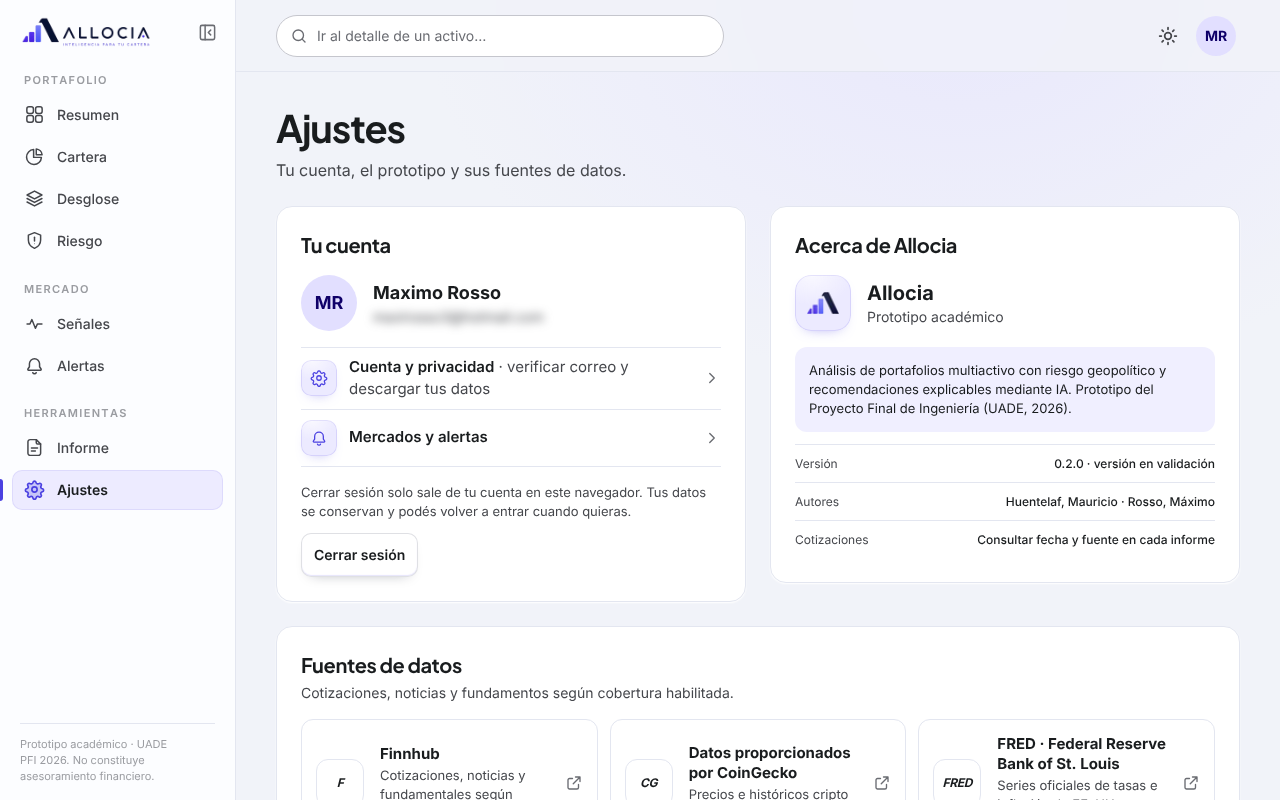
\includegraphics[width=0.82\textwidth]{figures/pantallas/web/a-09-ajustes.png}
	\caption{Captura de la pantalla de ajustes, con las fuentes de datos y el aviso del prototipo. Fuente: elaboración propia.}\label{fig:anx-ajustes}
\end{figure}

\section*{Wireframes del diseño original}
Los wireframes son anteriores a la implementación y tienen formato móvil. Cubren la bienvenida, el acceso y el registro (Figura~\ref{fig:wf-onboarding}), las secciones del diseño (Figuras~\ref{fig:wf-principales} y~\ref{fig:wf-senales}) y el desglose con el detalle por activo (Figura~\ref{fig:wf-detalle}). Alguna función que aparece en ellos, como la simulación de escenarios, se reemplazó durante la implementación por escenarios con fuentes (Subsección~\ref{sec:implementacion}).
\begin{figure}[ht]
	\centering
	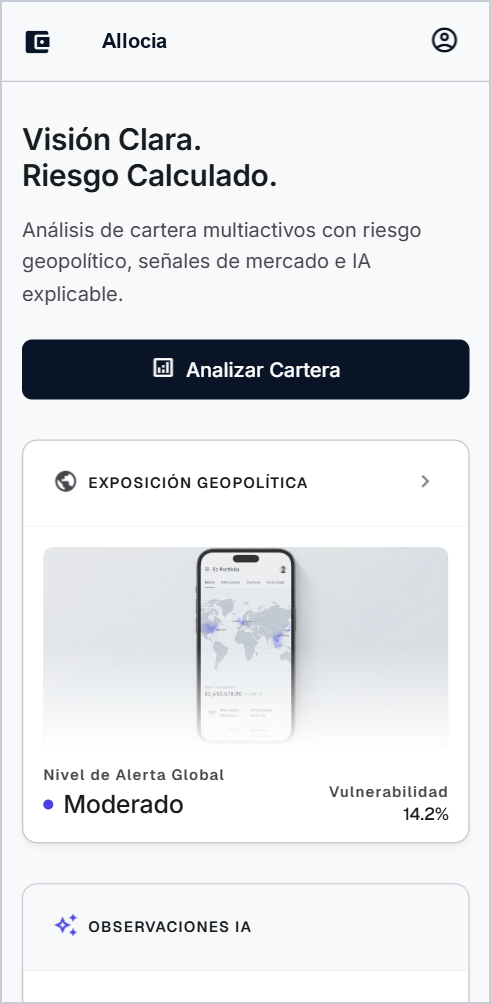
\includegraphics[height=9cm]{figures/wireframes/inicio.png}
	\hspace{0.35cm}
	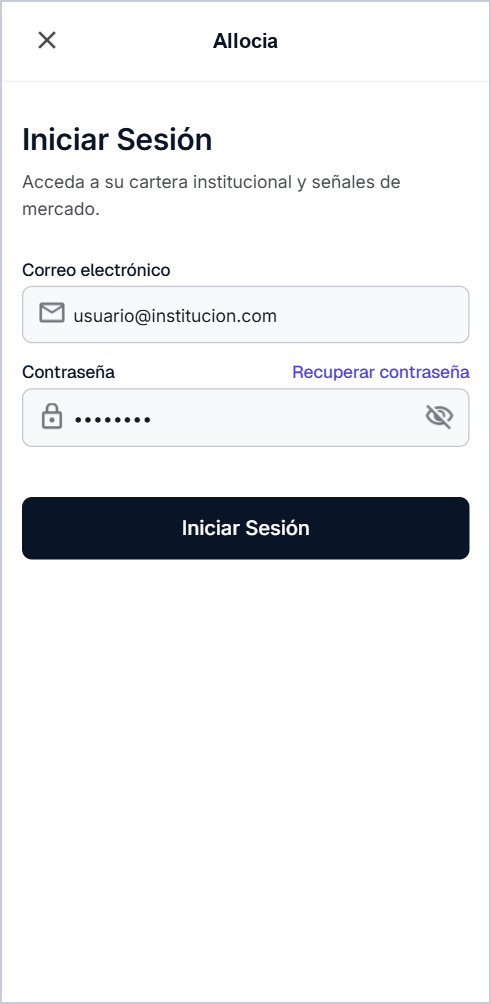
\includegraphics[height=9cm]{figures/wireframes/login.png}
	\hspace{0.35cm}
	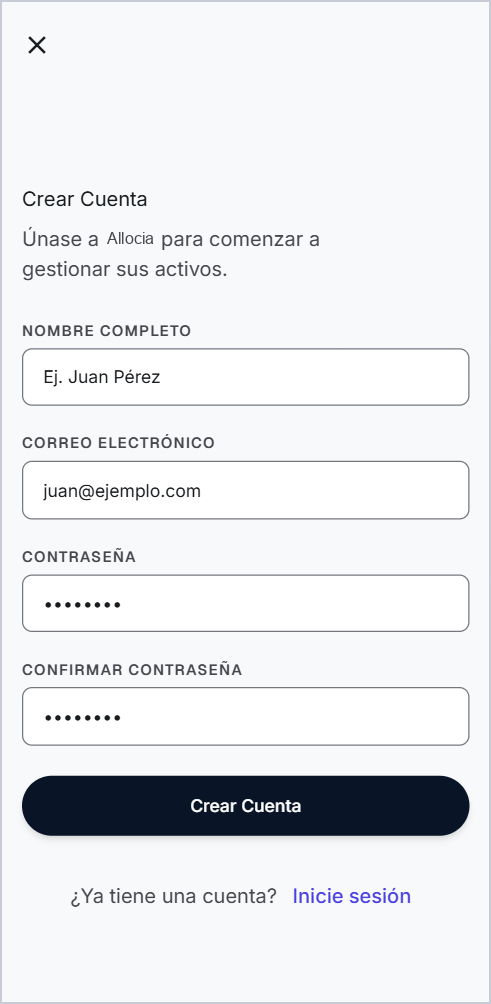
\includegraphics[height=9cm]{figures/wireframes/registro.png}
	\caption{Wireframes de bienvenida, inicio de sesión y registro (diseño de identidad). Fuente: elaboración propia.}
	\label{fig:wf-onboarding}
\end{figure}

\begin{figure}[ht]
	\centering
	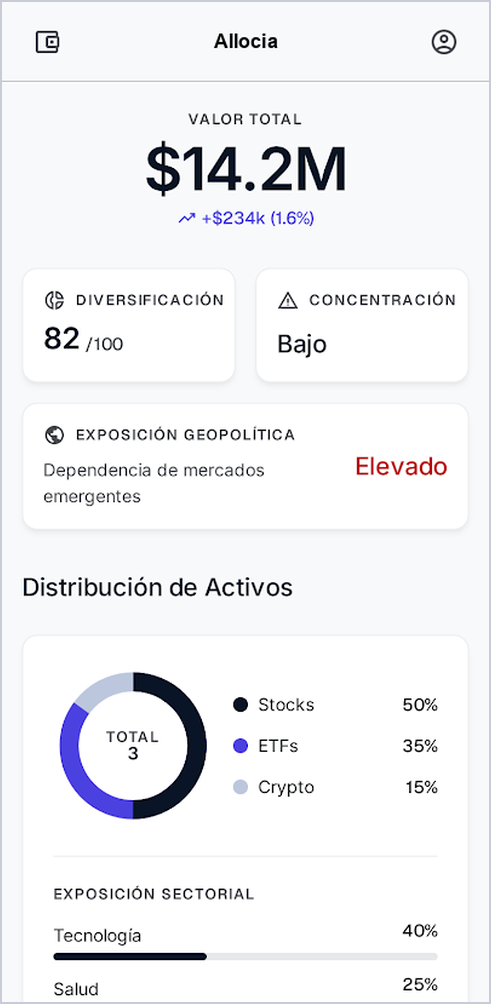
\includegraphics[height=9cm]{figures/wireframes/panel_principal.png}
	\hspace{0.35cm}
	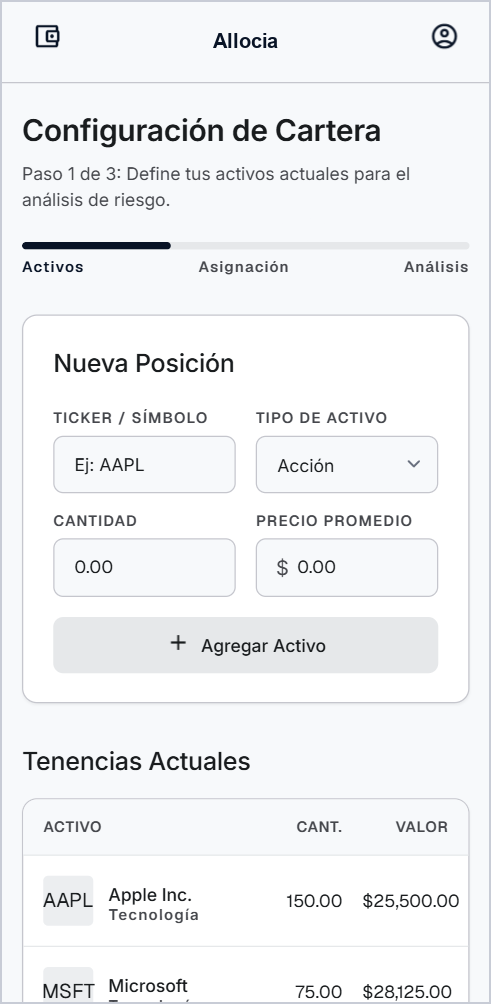
\includegraphics[height=9cm]{figures/wireframes/configuracion_cartera.png}
	\hspace{0.35cm}
	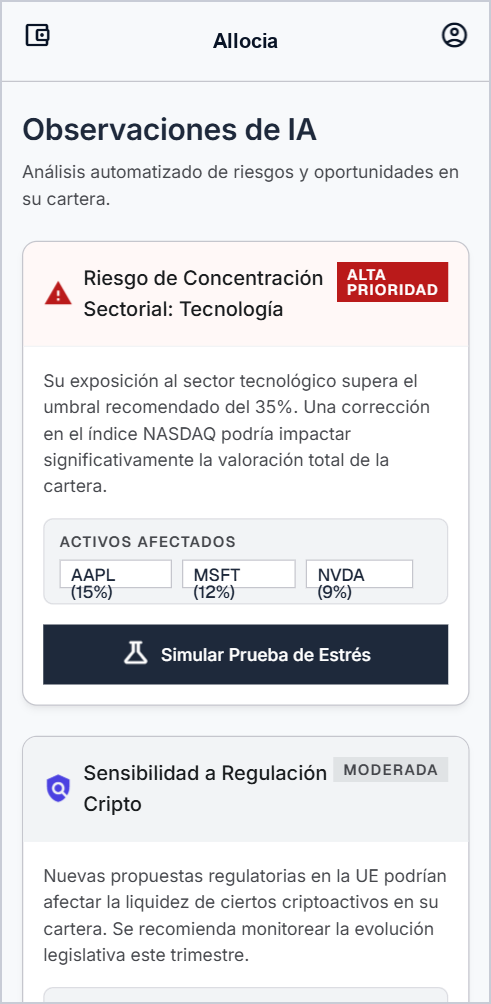
\includegraphics[height=9cm]{figures/wireframes/observaciones_ia.png}
	\caption{Wireframes de las secciones principales: panel de resumen, configuración de cartera y observaciones de IA. Fuente: elaboración propia.}
	\label{fig:wf-principales}
\end{figure}

\begin{figure}[ht]
	\centering
	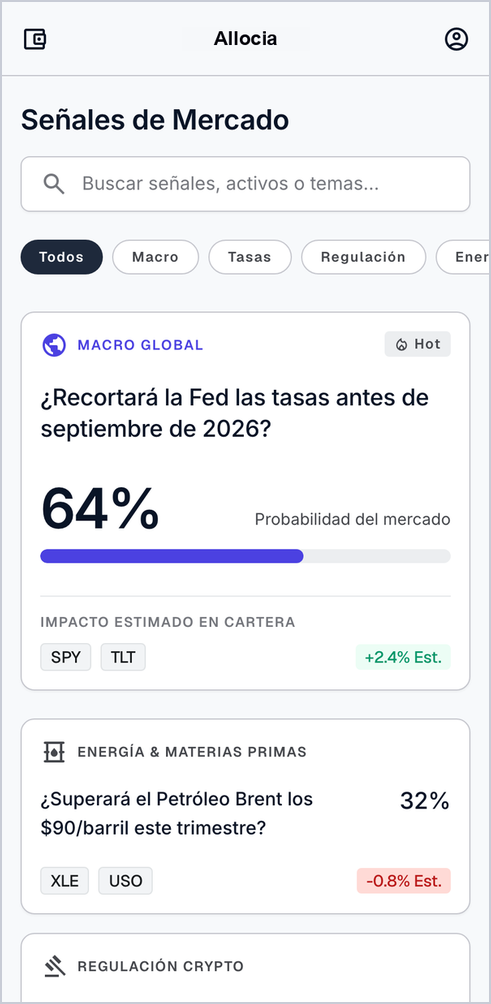
\includegraphics[height=9cm]{figures/wireframes/senales.png}
	\hspace{0.35cm}
	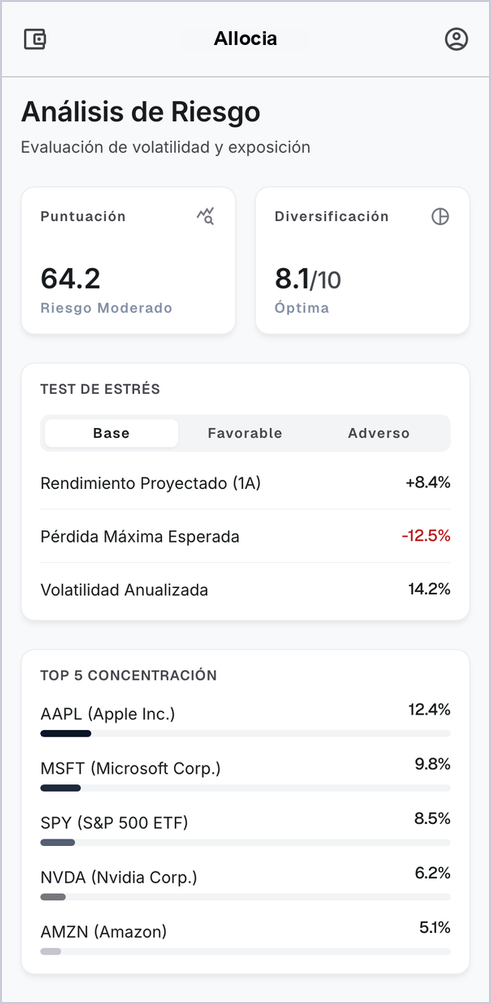
\includegraphics[height=9cm]{figures/wireframes/analisis_riesgo.png}
	\hspace{0.35cm}
	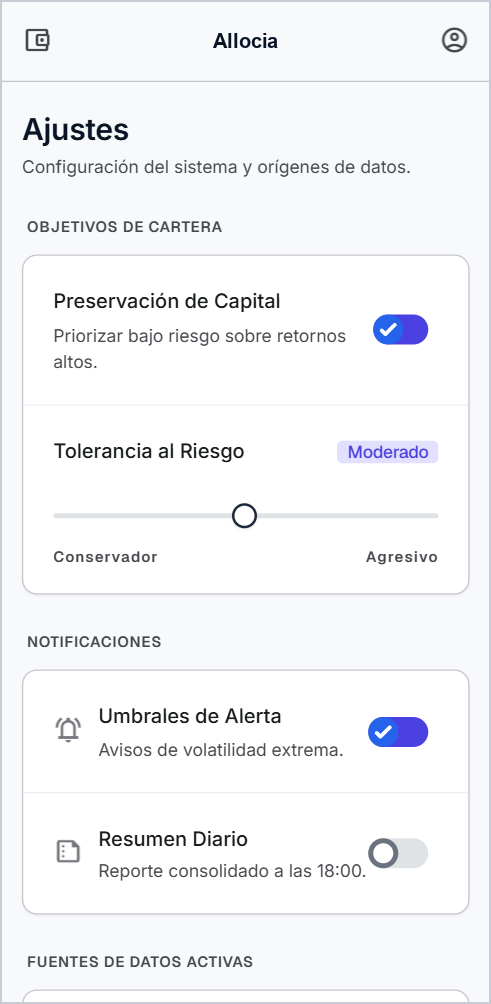
\includegraphics[height=9cm]{figures/wireframes/ajustes.png}
	\caption{Wireframes de señales de mercado, análisis de riesgo y ajustes. Fuente: elaboración propia.}
	\label{fig:wf-senales}
\end{figure}

\begin{figure}[ht]
	\centering
	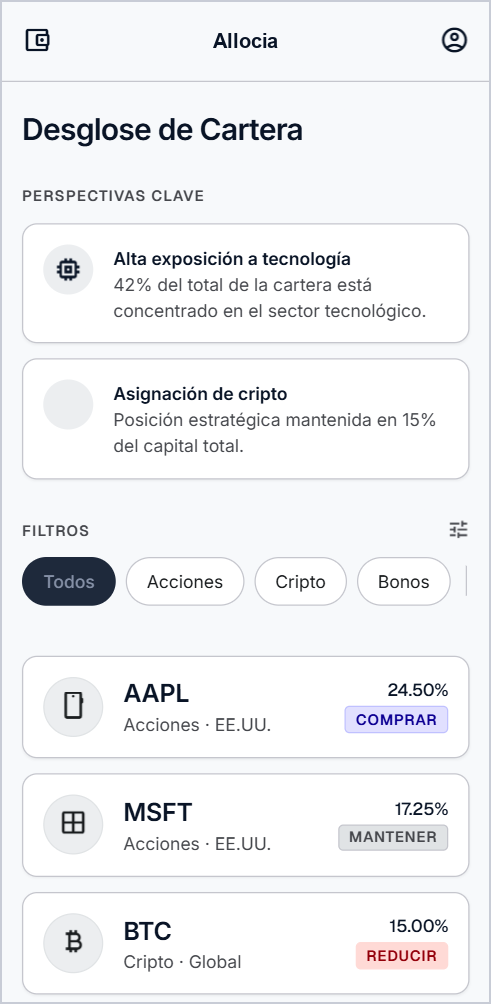
\includegraphics[height=9cm]{figures/wireframes/desglose.png}
	\hspace{0.35cm}
	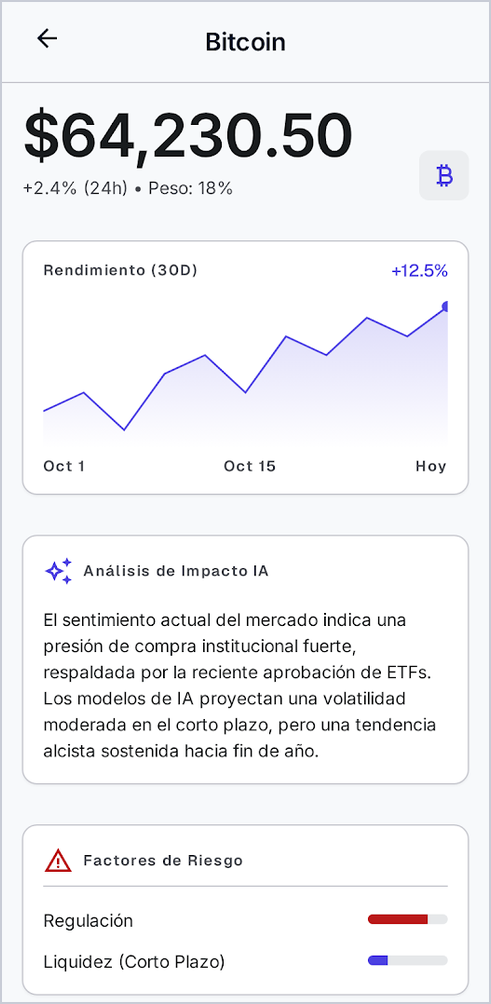
\includegraphics[height=9cm]{figures/wireframes/detalle.png}
	\caption{Wireframes de desglose de la cartera y detalle por activo. Fuente: elaboración propia.}
	\label{fig:wf-detalle}
\end{figure}

\section*{Privacidad y baja de cuenta en el diseño}
El diseño agrega, desde Ajustes, un acceso a la privacidad y a la eliminación de la cuenta. La Figura~\ref{fig:wf-privacidad} muestra el flujo que exigen RF9 y RF10, implementado y comprobado en el prototipo (Subsección~\ref{sec:pruebas-funcionales} y Subsubsección~\ref{sec:reverificacion-octubre13}); el esquema reproduce el diseño original. El aviso debe indicar responsable, finalidad, datos tratados, plazo de conservación y canal para ejercer derechos. La confirmación de baja debe explicar que se eliminan las posiciones y qué ocurre con las copias de seguridad según la política aplicable.
\begin{figure}[ht]\centering
\begin{tikzpicture}[box/.style={draw,rounded corners,text width=5.1cm,minimum height=5.5cm,align=left,inner sep=10pt,font=\small}]
\node[box,fill=blue!3] (a) {\textbf{Ajustes / Privacidad}\\[8pt]Datos de la cuenta.\\Finalidad del tratamiento.\\Conservación y derechos.\\Canal de contacto.\\[12pt]\fbox{Solicitar baja de cuenta}};
\node[box,fill=red!3,right=1cm of a] (b) {\textbf{Confirmar eliminación}\\[8pt]Cuenta y posiciones afectadas.\\Información sobre copias.\\Reautenticación.\\[12pt]\fbox{Cancelar}\\[8pt]\fbox{Confirmar eliminación}};
\draw[-{Stealth},thick] (a)--(b);
\end{tikzpicture}
\caption{Diseño del flujo de privacidad y baja. Fuente: elaboración propia.}\label{fig:wf-privacidad}
\end{figure}
